\chapter{Detecting Intruders}


\section{Preface}
The major problem faced during this work is related
to the detection of intruders while surveilling the house.
Modern security systems applies different techniques to detect intrusions
using many different sensors such as leap motion detection, face detection
or sound analysis. They have been working fine during the last years, however
thieves improves bypassing or partially avoiding these technique making the latter
less effective.\\
Therefore most of the work will be done investigating and testing innovative and
advanced techniques to deal with intrusions detection.

\section{Fingerprinting a Human}

During the time there has been many approaches to recognize a "Person"
using some of its peculiarities: software side with passwords or access phrases,
which should identify a single person; biometrics with finger prints, retina scans
and voice recognition.\\
Usually such controls where available only with expensive solutions (and some still are, e.g. retina
scanners), however with the introduction of \textit{IoT} their price dropped allowing
them to be sold for a reasonable price. These controls are also called \textbf{behavioral biometrics},
the set of behavioral traits which identifies an individual person. Usually these traits are
used for authentication when accessing a restricted system, however we'll consider
these to recognize unknown entities accessing our house. \\
These systems are mainly needed to prevent accidental triggering of the alarm, to be more
precise when listening or watching, not detecting just something but a real intrusion.

\subsection{Behavioral biometrics}
Detecting if someone in the house is someone familiar is not an easy task, most
of the approaches are precise in optimal conditions, much less when the situation
is non optimal (low light, low resolution etc). This impacts negatively their efficiency
when applied in a real life scenario, where usually the conditions are far from the optimal
situation. For example facial recognition works in very limited cases, like the systems
used on smartphones to unlock the device, has been reported to not be reliable enough
to be the main unlocking system. The situation is also similar for voice recognition or
speech to text systems, which are improving during the time and mainly \textbf{during the usage}.
\textit{Siri}, one of the most famous personal assistant had some minor troubles at the beginning
being used to the different users voices, accents and languages. \textit{Siri} uses
different voice recognition algorithms to categorize your voice by learning your
dictation and your accent, with good results over time.



\section{Expanding the system}
One of the biggest limitations of nowadays security system is their isolation
when installed. Most of devices are stand alone solutions incapable of extending
their functionalities to pre existing devices. If we want to expand \textit{Calvin} to
be adopted by others, including users and developers, we need to be able to extend its
functionalities with the ability to communicate with different other systems.

\section{The Architecture}

In this section we will go deep in the details of the architecture of the solutions
we propose.

\subsection{Accessing different systems}

Accessing different systems is a problem of technology interoperability between
different technologies running on architecturally different hardwares.
Most of the times \textit{IoT} devices runs on low limited power devices such as
an \textit{Arduino} or a \textit{Raspberry Pi}, both supporting different system
languages (the first is limited to a subset of \textit{C++} meanwhile the second one supports everything
that can run under a normal linux distribution, but usually it's \textit{Python}).
However in our scenario the devices we consider are on a different layer of abstraction,
we do target ecosystems and not single independent devices. \textbf{Ecosystems} has to
provide an access to developers through a point of access, \textbf{REST api} for   \textit{Nest}
and the \textbf{HomeKit.framework} for accessing \textit{HomeKit} devices.
The limitations are not always the same, when using \textit{Nest} it's easier to communicate
with it using a wrapper for their own api, which exists in many libraries, including \textit{Python}.
Nonetheless the situation with \textit{HomeKit} is much more strict, having their ecosystem
restricted only to their technology, \textit{Objective-C} or \textit{Swift}, which runs only
on \textit{Apple} branded device. Furthermore, the limitations are even more strict
due to the limitation of the framework only for \textit{iOS}, at the moment at least.
Usually the latter is the common case, which implies the need of a different solution
then "just wrapping" the apis in the code and plug them into the project.
In our case \textit{Calvin's} system is fully written in \textit{Python},
though it have many extension for a wide range of technologies, communicating
with \textit{HomeKit} is still hard to achieve.
In the following sections we'll describe the approaches taken to solve
the problem.




\section{Accessing Nest}

As said in the previous section \textit{Nest} has some advantages
due to their cloud apis, which makes it easier to reach the connected devices.

\subsection{Nest API Model}

\textit{Nest} offers a cloud API near real time, based on a subscription, that allows
users to build products accessing data on their devices, with the relative ability
to read and write data. With the \textit{Nest} cloud each element is identified as a resource
and accessible through a unique address, called "data location".
Furthermore, the cloud system also offers a \textit{RESTful} service to access these resources,
but only allowing GET and PUT operations with a call limit to prevent overuse. There is also
a \textbf{Streaming} feature for REST, which allows our application to receive updates
in real-time or to stream from a device, namely camera, since web-sockets are not supported.
However it applies the same rule as before, with some limits in the data usage to prevent abuse.

%%[TODO] maybe add some more description or api usage examples

However, the cloud functions of \textit{Nest} are limited to a restricted set of devices:
Thermostat, Protect (alarm), Camera and the Home.
Here are the functionalities offered by each of the products, with a brief description:
\begin{figure}[h]
\caption{Nest Cloud architecture}
\label{fig:nestarch}
\centering
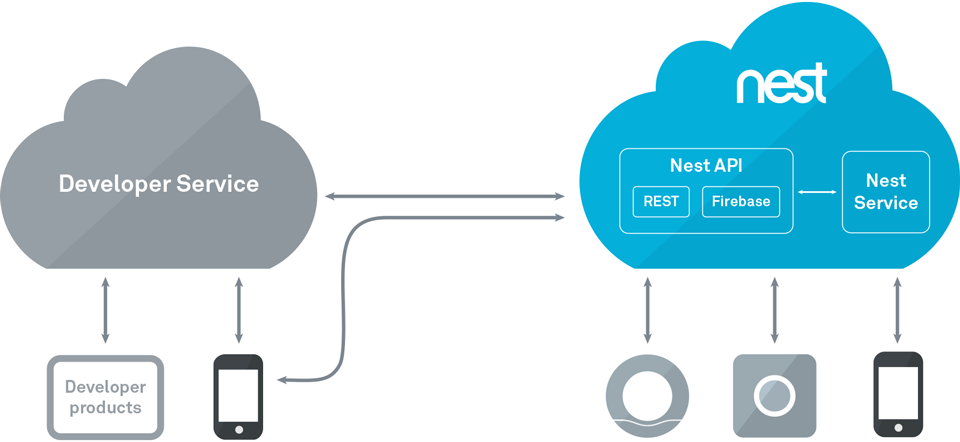
\includegraphics[scale=0.35]{nest-architecture.png}
\end{figure}

\subsubsection{Nest Thermostat}
Thermostat, as the name suggests, is a smart thermostat ,which can also be remotely controlled,
with some energy saving settings to help the user avoiding unnecessary heating expenses.   \\
Its remote functionalities are:

\begin{itemize}
    \item Read the current temperature
    \item Read or set a target temperature
    \item Set the fan timer
    \item Read or set the temperature mode
    \item See humidity values
    \item View online status and last connection information
    \item Read structure name and device location in the home
\end{itemize}

\subsubsection{Nest Protect}
Protect is a location based alarm for dangerous gas leaks, such as  Carbon monoxide \textit{CO}, or
smoke in case of fire.

\begin{itemize}
    \item View CO or smoke status
    \item View battery health state
    \item View last manual test status and timestamp for last manual test
    \item View online status and last connection information
    \item Structure name and device location in the home
\end{itemize}

\subsubsection{Nest Camera}
Camera, previously known as Dropcamera, is one of they key components of the
\textit{Nest} suite. It provides screen capture, audio and video streaming and the
other typical features offered by smart cameras.

\begin{itemize}
    \item View camera online status or mic status
    \item View or change streaming status (turn video streaming on/off)
    \item View device name and where identifier
    \item View last online status change (last online/offline change)
    \item View subscription status (enrolled/not enrolled)
    \item Learn more about Nest Aware with Video History subscriptions >
    \item View deep links to the live camera feed in the Nest app (iOS, Android) or on the web at home.nest.com
    \item View content related to the last event that triggered a notification, including:
        \\Sound or motion event detected
        \\Event start/stop times
    \item Deep links to image and gif files
    \item Structure name and device location in the home

\end{itemize}



\subsection{Nest with Calvin}

%%[TODO] create a nice chart to describe this
One of the key aspects of \textit{Calvin's} Actors is their abstraction
to allow their reuse in different situations. However, due to the different
nature of the ecosystem, specially \textit{Nest} and \textit{HomeKit} the actors
can't be used for the same purpose.
\textit{Nest} structure can be decomposed in two big sections: Structures and Devices.
Structure are objects to keep grouped together many devices, placing them in different part of the house,
but still not the most important part in our scenario.\\
A device is an abstraction of all the smart products offered by Nest, but mainly the one we have listed in the latter
paragraph.

\subsubsection{Device Abstraction}

We have abstracted a device in its most basic functions: setting and getting properties.
This simplification allows us to follow the best practices for the development of \textit{Calvin},
allowing a possible reuse of the actor. Here is the pseudocode for the high-level functions definition.

\begin{verbatim}
    getproperty: in device_id, property_name; out property_value
    setproperty: in device_id, property_name, value ; out True or False
\end{verbatim}


However going deeper into the actor architecture we have to define some more constraints,
like the events which trigger the execution and the tokens for which returning the results.
First of all, all incoming port of an actor has to be linked, we can not have an unbounded port,
both input or output. Here's a list of our actor's ports:\\

\begin{verbatim}
    Inputs:
        device: the device identifier
        operation: string representing the operation to do (get or set)
        property_name: the property to be get/set
        value: the value to be used to set the property
    Outputs:
        result: the property value
\end{verbatim}

To simplify the work, we reduced the inbound port for the operation to only one, instead of having a token
for a \textit{get} or \textit{set} operation. This task is completed using the \texttt{@condition} to declare
all the elements which are needed to fire and will be used in a particular action.
A simple condition for an action is the following example:
\begin{verbatim}
    @condition(action_input=['operation'], action_output=[])
\end{verbatim}
This condition requires the token operation to be bounded, and it will use it in its body function. Since
no \texttt{action\_output} is defined, the operation does not return any value.

Once all the inbound ports are connected, i.e. they have a token, the system will check the \texttt{@guard} condition,
which acts as a conditional control: it will continue only if the condition is satisfied.
An example guard condition can be written as:

\begin{verbatim}
    @guard(lambda self: self.nest._in_progress is None and self.operation == "set")
\end{verbatim}
This guard condition is used to enter the function only when the \textit{nest} object is not
working on an asynchronous task and the operation has to be the \textit{set} operation.\\
One of the constraints that an actor has to follow is the \textbf{reactivity}, which implies
non-blocking calls in the body of its functions. However, as in our case, the actor will have to
make some calls to the \textit{Nest} cloud, which is a blocking call. This is reached
using a two step asynchronous system: first the value is acquired and the actor
will delegate the request to a different thread; second when the delegate terminates it will
modify a flag to mark its completion, at that point the actor will return the value obtained
from the nest cloud. Asynchronous calls are needed since the scheduler loop can't be blocked
during the execution otherwise it would break the reactivity of the other actors.

\subsection{A Microservice Oriented approach}

Despite of the correctness of the former solution, it does however contains some
flaws in the architecture. The solution works with under the following circumstances:

\begin{enumerate}
    \item Libraries for connecting to a different ecosystem are provided in the same language (e.g. \textit{Python}).
    \item We assume the actor does never crash, and if it does the system may crash subsequently.
    \item The integration library won't require any change or modification in the future.
\end{enumerate}

However these assumptions are too risky to be considered for an always running system, because the likeliness
of one of the above problems to happen is very high.\\
To face these problems we adopted a \textbf{microservice} architecture style to implement the integration with
other ecosystems. In the case of \textit{Nest} is not very significative but it will be much more for \textit{HomeKit}, as
we'll see later.

\subsubsection{Microservice Architecture}


\begin{figure}[h]
\caption{Microservice Integration architecture}
\label{fig:test-arch}
\centering
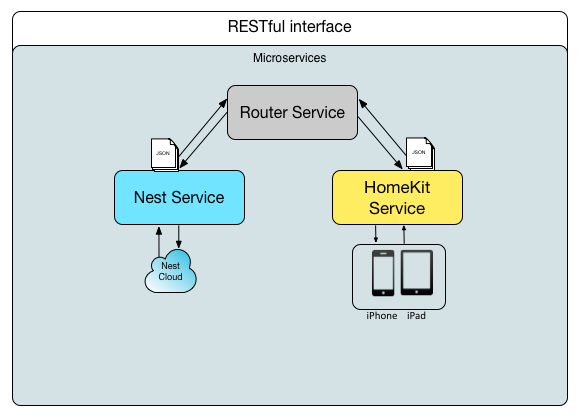
\includegraphics[scale=0.65]{test-arch.png}
\end{figure}

Figure \ref{fig:test-arch} illustrates the architecture proposed in our solution.
All the microservices can be reached through a router service, which doesn't expose
the real location of each service. This approach moves the service finding logic outside
of \textit{Calvin}, simplifying the work of the actor who won't have to deal with possible
re-deployments or re-locations of the service, it will just need to know where to reach the
routing service. This task will be deferred to the \textit{routing} service, which will act
as a proxy to the other micro-services.\\
Each ecosystem has a microservice dedicated, this is due to the different internal structure of the
different technologies. For example \textit{HomeKit} uses a hierarchical structure divided in the following,
from above to the bottom: \textbf{HMHome}, \textbf{HMRoom}, \textbf{HMAccessory}, \textbf{HMService} and \textbf{HMCharacteristic}.
Which differs from the simpler one of \textit{Nest}, where there are mostly Structures and Devices.\\
Moreover structuring the integration with ecosystems introduces the capability to link more accounts, more devices,
to the \textit{Calvin} runtime.

\subsubsection{The microservice API}

The API to describe the connection between \textit{Nest} and the microservice
resembles the former actor structure.
Following the classic \textit{RESTful} style, to access a device will look like
\begin{verbatim}
    Url
    GET /device/<deviceid>

    Example Response
    {"device":
        {
        "name": "DFF9", "temperature": 37, "humidity": 50, "fan": false,
        "mode": "heat", "online": false, "serial": "fake9396122EDFF9",
        "where": "basement","structure": "HomeTest", "target": 25
        }
    }

    [TODO] add all the other calls
\end{verbatim}





\subsection{Accessing HomeKit}

\textit{HomeKit}, introduced in details in the previous chapter, is the other ecosystem
for which we are extending \textit{Calvin} integration. First of all, HomeKit doesn't
expose any cloud API, it's functionalities can be accessed only through their \textbf{HomeKit.framework},
a library available only for \textit{iOS}. As can be seen the limitations compared to Nest
are much more strict, which implies no direct integration. The only possible solution for the
moment is to have an \textit{HTTP} web server exposing HomeKit functionalities to the outside of
the world. As previously mentioned, their library is not available on both \textbf{Mac OS X} nor
the Apple TV \textbf{tvOS}, which means the only possible approach is a mobile application.
However it is predicted to be supported by the former OS in the future, on which would be a more
elegant and nicer solution.\\

\subsubsection{Understanding}















\subsection{lol}
The answer is 42
